% Use only LaTeX2e, calling the article.cls class and 12-point type.

\documentclass[runningheads,a4paper]{llncs}

\usepackage[utf8]{inputenc}
\usepackage{amssymb}
\usepackage{amsmath}
\usepackage[draft]{hyperref}
\usepackage{graphicx}

 \setcounter{tocdepth}{3}

% Users of the {thebibliography} environment or BibTeX should use the
% scicite.sty package, downloadable from *Science* at
% www.sciencemag.org/about/authors/prep/TeX_help/ .
% This package should properly format in-text
% reference calls and reference-list numbers.

\usepackage{scicite}

% Use times if you have the font installed; otherwise, comment out the
% following line.

%\usepackage{times}

% The preamble here sets up a lot of new/revised commands and
% environments.  It's annoying, but please do *not* try to strip these
% out into a separate .sty file (which could lead to the loss of some
% information when we convert the file to other formats).  Instead, keep
% them in the preamble of your main LaTeX source file.


% The following parameters seem to provide a reasonable page setup.

%\topmargin 0.0cm
%\oddsidemargin 0.2cm
%\textwidth 16cm
%\textheight 21cm
%\footskip 1.0cm

\def\sectionautorefname{Section}
\def\tableautorefname{Table}
\def\figureautorefname{Figure}

% ACL style
%\setlength\columnsep{0.6cm}


%The next command sets up an environment for the abstract to your paper.

\newenvironment{sciabstract}{%
\begin{quote} \bf}
{\end{quote}}

% The following lines set up an environment for the last note in the
% reference list, which commonly includes acknowledgments of funding,
% help, etc.  It's intended for users of BibTeX or the {thebibliography}
% environment.  Users who are hand-coding their references at the end
% using a list environment such as {enumerate} can simply add another
% item at the end, and it will be numbered automatically.

\newcounter{lastnote}
\newenvironment{scilastnote}{%
\setcounter{lastnote}{\value{enumiv}}%
\addtocounter{lastnote}{+1}%
\begin{list}%
{\arabic{lastnote}.}
{\setlength{\leftmargin}{.22in}}
{\setlength{\labelsep}{.5em}}}
{\end{list}}


% Include your paper's title here

\title{
{\large \textnormal{Dissertation Proposal}} \\
Dialog Management with Deep Neural Networks
}

\titlerunning{Dialog Management with Deep Neural Networks}

% Place the author information here.  Please hand-code the contact
% information and notecalls; do *not* use \footnote commands.  Let the
% author contact information appear immediately below the author names
% as shown.  We would also prefer that you don't change the type-size
% settings shown here.

\author{Lukáš Žilka}
\urldef{\mailsa}\path{zilka@ufal.mff.cuni.cz}
\institute{
Institute of Formal and Applied Linguistics \\
Faculty of Matematics and Physics \\
Charles University in Prague \\
\mailsa\\
}

% Include the date command, but leave its argument blank.

\date{}



%%%%%%%%%%%%%%%%% END OF PREAMBLE %%%%%%%%%%%%%%%%



\begin{document}

% Double-space the manuscript.

%\baselineskip24pt

% Make the title.

\mainmatter

\maketitle

%\tableofcontents

%\newpage

\begin{abstract}
This document is a dissertation proposal submitted in partial fulfillment of the requirements for the doctoral exams. Its purpose is to define the dissertation goals and summarize initial experiments. We propose a novel approach to dialog state tracking in spoken dialog systems based on long short-term memory recurrent neural neural networks. The proposed model allows incremental, word-by-word dialog state tracking and is trainable from a corpus of annotated dialogs. The experiments show that the model achieves competitive performance on sub-tasks and suggest ways for improvement. Future work proposes extensions to the model and a way to use it for dialog state tracking with large knowledge-bases.
\end{abstract}
%{\footnotesize }

\section{Introduction}
%Voice is one of the most natural ways how people express themselves. Computer systems usually use graphic- or text-based interfaces for interaction, which are very effective . Spoken dialog systems are a special kind of computer systems designed to communicate with its users using voice. They started as simple dialog systems at help lines where

%Current spoken dialog systems consist of a pipeline of collaborating components.

A dialog state tracker is an essential component of modern spoken dialog systems. It maintains the user's goals throughout the dialog by looking at the automatic speech recognition (ASR) results of her utterances. For example, in the restaurant information domain, the dialog state tracker tracks what kind of food the user wants and which price range is she looking for, and provides this information as a probability distribution over \emph{food} and \emph{price\_range}: $\operatorname{P(\mbox{food}, \mbox{price\_range})}$ The dialog state tracker also needs to deal with speech recognition errors and tries to reduce their impact on the dialog~\cite{williams2013dialog}.

The standard mode of operation of a spoken dialog system is turn-by-turn, where the system always waits for the user to stop talking and only then generates its response. Also the system assumes its responses are spoken to the user as a whole without interruption. This brings simplicity to the spoken dialog system architecture, because the system can be implemented as a pipeline without feedback loops, but it also introduces some limitations. Particularly, people are used to say feedback things during the system's response as a sign of understanding, surprise or not-understanding, like ``yes'', ``ok'', ``really'', or ``oh, wait''. Also, sometimes only partial information provided by the system is enough for the user, and she will interrupt the system in the middle of its utterance to ask a follow-up question or otherwise continue with the dialog. The turn-by-turn mode of operation does not allow for utilizing these clues. We will refer to the more advanced mode of operation, where the system processes the user's input incrementally as it is coming in and also generates the response incrementally, as word-by-word. This mode of operation allows the dialog system to be more natural and responsive with the user, because it can interpret the various signs the user gives during the system's responses and react more precisely to what the user says. A simple example of a dialog system working in this advanced mode can be found in~\cite{skantze2009incremental}.

The state-of-the-art dialog state trackers~\cite{williams2014web,henderson2014word,lee2014optimizing,smith2014comparative,sun2014sjtu} achieve their performance by learning from annotated data, and they were shown to work well in the restaurant information domain in the dialog state tracking challenge DSTC2~\cite{henderson2014second}. However, they possess two undesirable traits. First, they can only track the dialog state turn-by-turn (as opposed to the more complicated word-by-word approach), which limits the responsiveness of the dialog system. Second, some of the trackers rely on the results from a spoken language understanding (SLU) component~\cite{wang2005spoken}, which brings an additional component into the dialog system that needs to be trained and tuned. In this thesis proposal we aim to address these problems.

The contribution of this thesis proposal is a novel approach to dialog state tracking.
It aims towards building more responsive and simpler dialog systems by proposing the first trainable dialog state tracker which naturally operates incrementally, word-by-word, and can directly learn from annotated dialogs, removing the need for an SLU unit. The word-by-word mode of tracking allows the dialog manager to be more responsive with the users. Simplicity comes from the fact that the whole dialog state tracker can be automatically optimized from data by a standard backpropagation algorithm.

Our approach is based on the modern deep learning techinques, particularly the long-short term memory recurrent neural network (LSTM RNN)~\cite{hochreiter1997long}.
We have chosen this approach due to several reasons:
First, LSTMs were shown to be effective for learning sequence mappings in automatic speech recognition~\cite{graves2005framewise}, machine translation~\cite{sutskever2014sequence}, protein structure prediction~\cite{sonderby2014protein}, and many other sequence classification tasks. The length of the sequences successfully modelled by LSTMs is comparable to the length to the word sequences in the spoken dialog systems.
Second, the sequential nature of the dialog naturally fits the LSTM's recurrent mode of operation. And finally, as the tracker processes the input, it incrementally builds an intermediate representation of the dialog. It has been shown that good intermediate representations help generalization~\cite{gulccehre2013knowledge}.
The success of LSTM on multiple complicated and diverse tasks promises to be exploitable also in dialog state tracking.

%In the thesis proposal we explore several directions towards dialog state tracking with LSTM networks:
%\begin{itemize}
%  \item 1-best LSTM-based dialog state tracker
%  \item n-best LSTM-based dialog state tracker
%  \item Attention-based dialog state tracker.
%  \item Reinforcement learning-based dialog state tracker.
%\end{itemize}

The thesis proposal is organized as follows. First, we give an overview of the relevant spoken dialog systems and neural networks literature (\autoref{sec:background}). In \autoref{sec:lstm_dialog_state_tracker}, the model of the LSTM dialog state tracker is described along with the experiments. In \autoref{sec:future_work}, we discuss the future research directions.


\section{Background}
\label{sec:background}
This thesis builds upon the work from the fields of statistical spoken dialog systems and deep neural networks.

\subsection{Spoken Dialog Systems}
\label{sec:spoken_dialog_systems}
A spoken dialog system needs to understand what the user says, process it and provide an answer. Usually the dialog systems are turn-based, meaning that the system listens to the user and only replies when the user stops talking~\cite{thomson2010bayesian}. They are commonly built as a pipeline of several components:
\begin{enumerate}
  \item The automatic speech recognition (ASR) component converts the user's speech to text.
  \item The spoken language understanding component converts the text into structured information.
  \item The dialog management component updates the dialog state and generates a system action.
  \item The structured system action is converted to natural text.
  \item The natural text is synthesized and spoken back to the user.
\end{enumerate}

\subsubsection{Automatic Speech Recognition}
The task of an automatic speech recognizer is to decode the user's utterance into a structure called \emph{ASR hypothesis}. Typically the hypothesis is either an 1-best list~\cite{gorin1997may,wang2003word}, an n-best list~\cite{he2003data}, a word confusion network\cite{hakkani2006beyond} or a word lattice~\cite{oerder1993word}. Word lattices are the richest but also the most complex structures to work with. It has been shown that using word lattices or word confusion networks in the spoken language understanding yields substantially better results over 1-best hypothesis~\cite{tur2002improving}. The ASR hypothesis is consumed by the other components of the dialog system.

There are open-source and commercial ASR solutions available with varying capabilities and purposes of use. The most pouplar open-source solution is Kaldi~\cite{povey2011kaldi}, which can be trained out-of-the-box to provide state-of-the-art ASR performance. Google Speech API\footnote{https://www.google.com/intl/en/chrome/demos/speech.html} is a popular commercial solution that is very fast and accurate for general speech and supports a lot of languages, but is not customizable and has unclear licensing conditions. Nuance's\footnote{http://dragonmobile.nuancemobiledeveloper.com/public/} commercial recognizers are more flexible but they are paid and closed-source. ISpeech ASR API\footnote{http://www.ispeech.org/api} is also customizable (users can select expected speech type: text messages, voice mail, dictation) but it does not allow full customization and is also paid. AT\&T Watson\footnote{http://developer.att.com/apis/speech} allows users to provide a custom grammar (language model) but
its free use is limited.

\subsubsection{Spoken Language Understanding}
Spoken language understanding (SLU) unit aims to interpret the user's intention from their speech utterance~\cite{wang2005spoken}. Particularly it converts the ASR hypothesis to some form of meaning representation. For example ``yes'' could be represented as ``affirm()'', or ``I want to go to Brno'' as ``inform(task=find\_connection)\&inform(to\_stop=Brno)'' in the meaning representation used in the ALEX dialog system~\cite{duvsek2014alex}. The meaning representation is arbitrary and adjusted to the particular dialog system. Examples of other representations can be found in~\cite{skantze2008galatea,he2003data}.

Historically, SLU has been done by manually writing grammars used to fill slots in semantic frames~\cite{ward1994recent,dowding1993gemini}, but this is expensive and non-flexible, because an expert needs to devise the grammar and then laborously maintain it. As the complexity of the domain grows the maintanence effort grows much more. Instead, statistical approach to SLU has been adopted, where SLU is viewed as a pattern recognition problem
$$\hat M=\operatorname{arg~max}_M \operatorname{P}(M|W)$$
where we are looking for the best meaning representation $M$ of the input given the ASR hypothesis $W$. The main benefit of this approach is the ability of the model to leverage the training data to improve its performance. HMM can be used to model the joint probability of the words and meaning representation given the acoustic signal~\cite{pieraccini1992progress,pieraccini1992stochastic}. Hidden Vector State model that learns stack operations to parse the user's utterance in a hierarchical way was proposed~\cite{he2003data}. It is particularly appealing for its ability to infer the hierarchy in the user's utterances without explicit hierarchical annotations. Markov Logic Networks were used for SLU by~\cite{meza2008spoken}, where first-order logic formulaes are used as templates to instantiate complex Markov network that model the slot-value representation. In~\cite{zettlemoyer2007online} an algorithm that learns to parse the text input into lambda-calculus expressions using extended combinatory categorial grammar is given.

\subsubsection{Dialog Management}
Dialog management (DM) component directly influences how natural and intelligent will the dialog system be perceived among its users. Its task is to come up with the next action of the system given the previous progress of the dialog. It usually consists of two parts: dialog state tracking, and dialog policy.

Dialog state tracking watches the dialog progress and keeps track of important information in form of the dialog state, or as a probability distribution over all possible dialog states called the belief state. Usually, the dialog state is a structure that contains several components that take several values, for example a component ``food'' that can take values ``chinese'', ``indian'', or ``thai'', and a component ``area'' that take values ``north'' and ``south'', and usually only the information needed for the dialog policy is tracked.

Dialog policy acts upon the dialog state or the belief state to generate the next action. There are handcrafted approaches to the dialog policy~\cite{pieraccini2005we,skantze2008galatea}, and approaches that automatically learn from observing rewards~\cite{levin2000stochastic,walker2000application,lemon2006isu,thomson2010bayesian}.

\paragraph*{Bayesian Networks}
Bayesian networks can be used for the belief state tracking~\cite{pulman1996conversational,williams2007applying,bui2006tractable,thomson2010bayesian}. The belief $b$ is updated as
$$b'(s)=\frac{1}{Z} \cdot P(o'|s,a)\sum_{s'}P(s|s',a)b(s')$$
where $o$ is the observation, typically the user utterance, $s$ is the dialog state and $a$ is the system action.

\paragraph*{Recurrent Neural Network Tracker}
Using recurrent neural network (RNN) for dialog state tracking has been proposed in~\cite{henderson2014word,henderson2013deep}. N-gram features from n-best lists are extracted and used as an input to the RNN model at each turn. The hidden state is updated for each slot as
$$h_t=f(x_t, h_{t-1})$$
where $h_t=(p_t, m_t)$ consists of the distribution over the slot's values in form of the vector $p_t$ and memory $m_t$.

\paragraph*{Ranking-based Tracking}
The dialog state tracking was posed as a ranking problem by~\cite{williams2014web}, where all the possible dialog states given the observed SLU hypotheses so far are enumerated and then ranked using a LambdaMART ranking algorithm. Then the best ranked dialog state is selected as the hypothesis.

\paragraph*{Discriminative Model Tracking}
Generalized linear regression model $f$ was trained to update the belief state
$$b'(s)=f(b(s), a, o)$$
and shown to outperfrom heuristic update rules~\cite{bohus2006k}.

\subsubsection{Natural Language Generation}
The natural language generation (NLG) component generates the natural language utterance of the system action generated by DM. For example, if the system generates the action \texttt{confirm(food=chinese)} then the NLG should generate ``Did you say chinese food?''. The simplest approach is a template-based NLG that has a database of templates, where for each possible system action there is a template to be used~\cite{duvsek2014alex}. A more sophisticated approach is a data-driven model that given a corpus of (system action; its surface realization; alignment) tuples learns to generate the natural language utterances~\cite{mairesse2010phrase}.

\subsubsection{Speech Synthesis}
Speech synthesis takes the natural language utterance generated by NLG and transforms it to speech signal. Two main approaches are used: 1.) concenative speech synthesis~\cite{campbell1997prosody,masuko1996speech}, and 2.) statistical parametric speech synthesis~\cite{zen2009statistical} Users still consider the concenative approach to be better, but the statistical parametric speech synthesis is catching up quickly~\cite{zen2009statistical}.

The concenative speech synthesis (also called unit-selection synthesis) uses a database of speech segments, from which it selects some and concatenates them together to form the speech signal. The input utterance is converted to a sequence of speech units that describe how it should be pronounced. For each speech unit the synthesizer finds the most appropriate segment from the database, in terms of the similarity to the sound to be synthesized speech unit and the smoothness of concatenation with the other segments.

Statistical parametric speech synthesis directly models the acoustics of the speech. During the training of the model, linguistic $l$ and acoustic features $a$ are extracted from the training data and a conditional model of $p(a|l)$ found. During synthesis the best acoustic features for the given linguistics features are found $\hat{a}=\operatorname{arg~max}_a p(a|l)$. HMM\cite{yoshimuray1999simultaneous}, DNN~\cite{ze2013statistical}, and RNN~\cite{zen2015unidirectional} were used as the conditional models.

\subsection{Deep Neural Networks}
Neural networks are known to be universal function approximators~\cite{hornik1989multilayer}, thus are able to model arbitrary measurable function with arbitrary accuracy given enough capacity. Thanks to the never-ending advances in the computational speed, which brought computer architectures capable of coping with previously inconceivable amounts of data, and thanks to the fact that the neural networks have enough capacity to leverage this data, the new neural networks applications were able to achieve impressive results on various tasks. New applications of neural networks in almost all fields where machine learning was applied before yielded the new state-of-the-art results or came close to the state-of-the-art performance with much simpler models (e.g. automatic speech recognition~\cite{graves2005framewise}, machine translation~\cite{sutskever2014sequence}, image recognition~\cite{karpathy2014deep}, natural language processing~\cite{socher2012semantic}, protein structure prediction~\cite{sonderby2014protein}). Also because the fundamental algorithm that underlies the deep learning, the gradient descent algorithm, is very simple and computationally tractable, it allowed the researches to build bigger and better models. Proving once again that simple models with more data beat more complex models~\cite{halevy2009unreasonable}.

The research in the deep neural networks is also fueled by the available open-source deep learning toolkits like Theano~\cite{bastien2012theano}, Torch7~\cite{collobert2011torch7}, or Caffe~\cite{jia2014caffe}, that provide a good programming infrastructure for building custom neural network models and for testing hypotheses fast. With these toolkits it is very easy to share experimental code, try out new models, and replicate experiments.
% TODO: Maybe describe each more?

The currently used neural networks are called deep because of their architecutre. It consists of several layers of parametrized computational units. We can classify the deep neural networks by their architecture into several conceptual classes:
\begin{itemize}
  \item fully-connected networks -- their layers are densely connected and their input is just a vector $x$ that is mapped to output $y=f(x)=g(W\cdot x)$, where $g(.)$ is some activation function like $\operatorname{tanh}$, $\operatorname{\sigma}$, or $\operatorname{ReLU}$, and $W\in \mathbb{R}^2$ is a matrix of parameters
  \item convolutional networks -- their layers are connected through a convolutional kernel; the convolutional kernel behaves like a small fully-connected layer applied at the different positions of the input simultaniously $y_1=f(x_{1:|k|})$, ..., $y_{n-|k|+1}=f(x_{n-|k|+1:n})$; the result is usually very large so it is transformed by a pooling layer into a smaller space $y=\operatorname{pool}(y_1, ..., y_{n-|k|+1})$; in the most general case the pooling layer sub-samples its inputs, for example selects the maximum values for each dimension of the input vectors
  \item recurrent neural networks -- are almost the same as the fully-connected networks, but with the difference that they are applied to a sequence rather than a single input $x_1$, $x_2$, ..., one by one, and some of the results of the computation performed by computing an output for the input $x_t$ (e.g. the values of the hidden layer) are passed on to the function's application on the next element of the sequence $x_{t+1}$; formally we have $(y_i, h_i) = f(x_i, h_{i-1})$, where $h_i$ denotes the results of the computation passed from the previous step, and $y_i$ is an output
\end{itemize}
However, this classification is not strict and almost every model from the literature is a combination of these classes. We aimed to give an intuitive feel for the different classes of architecture rather than their rigorous description, which can be found in the literature~\cite{graves2013generating}.
% TODO: Describe each of the classes.

\subsubsection{Long Short-Term Memory Networks}
\label{sec:lstm}
An important type of the recurrent neural networks is the long short-term memory (LSTM)~\cite{hochreiter1997long} model that aims to overcome some of the practical drawbacks of the standard RNN model. Standard RNN model suffers from the vanishing gradient problem~\cite{bengio1994learning} during training, and also the network forgets information very fast. LSTM's special architecture aims to overcome this, and has the following form:
\begin{align*}
\bf{f}: & X \times U \rightarrow U \\ %x_t, (h_{t-1}; c_{t-1}) \rightarrow
f(x_t, u_{t-1}) & = u_t = \begin{pmatrix}
h_t \\
c_t
\end{pmatrix} \\
i_t &= \sigma(\operatorname{W_{(i)}} \cdot \begin{pmatrix}
x_t \\
h_{t-1}
\end{pmatrix} + b_{(i)}) \\
f_t &= \sigma(\operatorname{W_{(f)}} \cdot \begin{pmatrix}
x_t \\
h_{t-1}
\end{pmatrix} + b_{(f)}) \\
x'_t &= \operatorname{tanh}(\operatorname{W_{(x)}} \cdot \begin{pmatrix}
x_t \\
h_{t-1}
\end{pmatrix} + b_{(x)}) \\
c_t &= f_t \odot c_{t-1} + i_t \odot x'_t \\
o_t &= \sigma(\operatorname{W_{(o)}} \cdot \begin{pmatrix}
x_t \\
h_{t-1}
\end{pmatrix} + b_{(o)}) \\
h_t &= o_t \cdot \operatorname{tanh}(c_t)
\end{align*}

The vectors $i_t, f_t, o_t$ represent the input, forget and output gates, respectivelly, $x'_t$ is the modulated input, the vector $c_t$ is the cell state and the vector $h_t$ denotes the output, jointly denoted by $u_t$.

\section{LSTM Dialog State Tracker}
\label{sec:lstm_dialog_state_tracker}
In this section we will describe our dialog state tracking model based on the long short-term memory units. Our model fits in the big picture of a spoken dialog system described in~\autoref{sec:spoken_dialog_systems} as a spoken language understanding and dialog state tracker together. Thus it connects between the automatic speech recognizer, getting the ASR hypotheses as its input and provides the belief state as its output to the dialog policy.

Particularly, the task of our tracker is to map a sequence of words in the dialog $w_1$, ..., $w_t$ to predictions for each of the $k$ dialog state components $(p^{(1)}_t, ..., p^{(k)}_t)$. Each $p^{(i)}_t$ is a vector corresponding to a probability distribution over the values of the i-th dialog state component. For example, $p^{(area)}_t$ is a probability distribution over values $\{north, south, east, west\}$ at the time $t$.

%The task of dialog state tracking is to monitor progress in the dialog and provide a compact representation of the dialog history in the form of a \emph{dialog state}~\cite{henderson2014second,zilka2013comparison}. Because of uncertainty in the user input, statistical dialog trackers maintain a probability distribution over all dialog states, called the \emph{belief state}. As the dialog progresses, the dialog state tracker updates this distribution given new observations.
\subsection{Dialog State}
In this thesis, we define the dialog state at time $t$ as a vector $s_t \in C_1 \times ... \times C_k$ of $k$ dialog state components, sometimes called slots. Each component $c_i \in C_i=\{v_1, ..., v_{n_i}\}$ takes one of the $n_i$ values. Our dialog state tracker maintains a probability distribution over $s_t$ factorized by the dialog state components:
$$P(s_t|w_1, ..., w_t)=\prod_i p(c_i|w_1, ..., w_t; \theta)$$

Note that all models $p(c_i|\cdot)$ share a substantial portion of the parameters, as detailed in the next section, so despite the fact that the predictions are factorized and thus independent, they were optimized to minimize a joint objective function and therefore naturally model the dependence between the dialog state components.

\subsection{Model}
Our dialog state tracking model can be seen as an encoder-classifier model, where an LSTM is used to encode the information from the input word sequence into a fixed-length vector representation. Given this representation, the classifier produces a probability distribution for each of the dialog state components.

Formally we have an encoder that maps an input word and a previous hidden state to a new hidden state, $Enc(w, h_{t-1})=h_t$, and a classifier that maps a hidden state to a prediction, $C(h_t)=p_t$. To encode the whole dialog, the encoder is applied sequentially on the input sequence of words. In our system, we have one encoder $Enc$ and multiple classifiers $C$, one for each dialog state component (e.g. $C^{(food)}$, $C^{(area)}$, ...).

The model of the encoder $Enc$ is a LSTM RNN (as described in~\autoref{sec:lstm}). In case of a recursive application of $Enc$, we write $Enc(w_1, ..., w_n, h, c)$ instead of $Enc(w_n, ... Enc(w_1, h, c))$ to simplify the notation. The model of the classifier $C$ is a single-layer neural network with rectified linear units in the hidden layer and the softmax output layer. The architecture is illustrated in~\autoref{fig:LecTrack}.

\begin{figure*}
\center
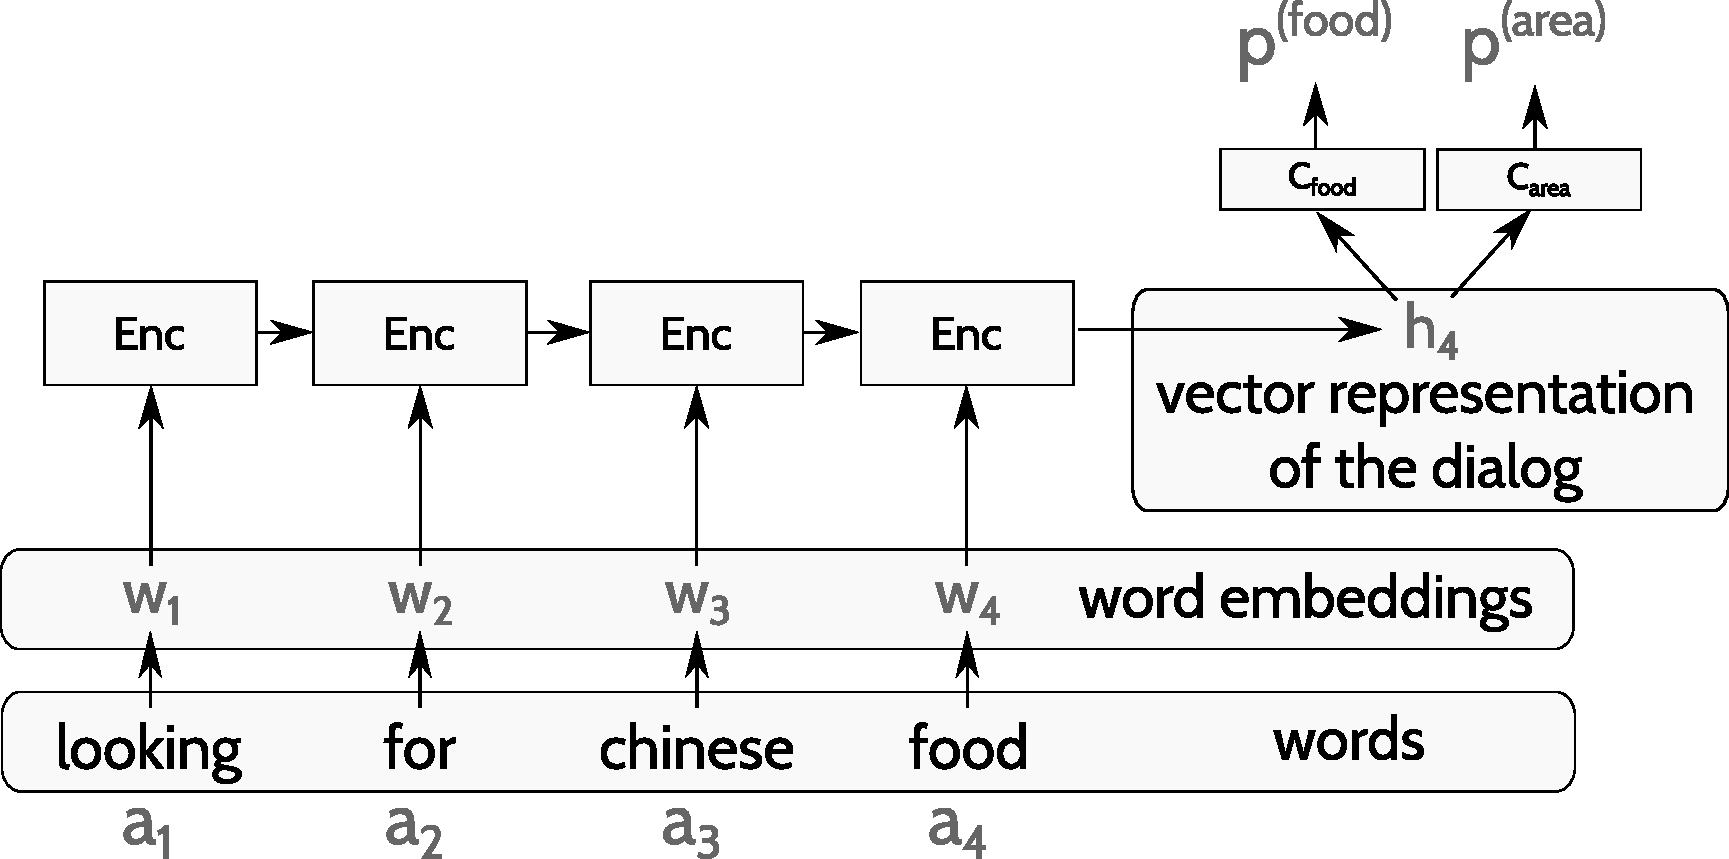
\includegraphics[width=0.75\textwidth]{arch}
\caption{A demonstration of the LSTM Dialog State Tracker applied to a user utterance ``looking for chinese food''. The encoding LSTM model $Enc$ is sequentially applied to each input word and at the end, its hidden state is used to feed to the state component classifiers.}
\label{fig:LecTrack}
\end{figure*}

The encoder and classifier form together the LSTM dialog state tracker that we call \emph{LecTrack}:
\begin{align*}
\bf{LecTrack}: & ~a_1, ..., a_n \rightarrow p_{1}, ..., p_{k} \\
\forall i \in {1, ..., k}: & ~p_i = \operatorname{C_i}(\operatorname{Enc}(E \cdot a_1, ..., E \cdot a_n, h_0, c_0))
\end{align*}
Here, $n$ is the length of the input sequence, $k$ the number of the dialog state components, $a_1$, ..., $a_n$ is the input word sequence encoded in a one-hot encoding, $E$ is a word embedding matrix, and $h_0=c_0=\bf{0}$ are zero vectors. As shown, each token $a_i$ is mapped to its corresponding embedding vector through the embedding matrix $E$, $w_i=E\cdot a_i$. The literature suggests many ways for obtaining the embedding matrix $E$~\cite{mikolov2013efficient,kim2014convolutional,stratosspectral}, but in the experiments in this thesis, we treat it just as another set of parameters for the sake of simplicity.\footnote{Informal experiments with different types of initialisaion of word embedings, such as using word2vec~\cite{mikolov2013efficient} embedings estimated from a large out-of-domain corpus, did not suggest any advantage over randomly initialised embeddings in this relatively limited domain. Therefore, we decided not to explore this direction further.}

\subsection{Training}
The model is trained using the standard cross-entropy criterion~\cite{rubinstein2004cross} in the vanilla stochastic gradient descent scenario~\cite{bottou2010large}:
$$ l(a_1, ..., a_n, y_1, ..., y_k; \theta) = \sum_{i=0}^k \operatorname{log} \operatorname{LecTrack}(a_1, ..., a_n)^i_{y_i}$$
Here, $\operatorname{LecTrack}(.)^m_n$ denotes the probability of the $n$-th value in the $m$-th dialog state component.

After each optimization epoch, we monitor the performance~\footnote{See the experiments section for the description of the featured metrics.} of the model on a held-out set $D$. When the performance stops increasing for several iterations, we terminate the training and select the best-performing model.


\subsection{Experiments}
\label{sec:experiments}
\subsubsection{Dataset}
To train and evaluate our model, we use the DSTC2~\cite{henderson2014second} data, which is a common data set for dialog state tracking evaluation. The DSTC2 data consists of about 3,000 dialogs from the restaurant information domain, each dialog is 10 turns long on average. The data is split into training, development and test sets. This data allows us to measure the performance of our tracker on turn-based dialogs. Ideally we would run the evaluation on a dataset where we could also measure the incremental capabilities of the tracker, but to the best of our knowledge, no such dataset is publicly available yet, and we shall address this in our future work.

\subsubsection{Baseline}
A baseline system for this domain has been provided by the DSTC2 organizers. It uses the SLU results and confidence to rank hypotheses for the values of the individual dialog state components. There were several baselines described in~\cite{henderson2014second} and we report the results of the \emph{focus} baseline, which was the best among them.

\subsubsection{Data Preprocessing}
Each dialog turn contains the system utterance and the user utterances, which we need to serialize into a stream of words as the input to our model. The system utterance undergoes a simple preprocessing detailed below, and the user utterance is directly fed to the model word-by-word without any further preprocessing. There is no difference between the system and user utterance in the eyes of our model, both are seen together as one long sequence of words.

\paragraph*{System Input:}
To get the the system input, we perform a simple preprocessing. We flatten the system dialog acts of the form \texttt{act\_type(slot\_name=slot\_value)} into a sequence of two tokens $t_1, t_2$, where $t_1=(\operatorname{act\_type}, \operatorname{slot\_name})$ and $t_2=\operatorname{slot\_value}$. For example \texttt{request(slot=food)} is flattened as $(request, slot), food$, which the model then sees as a word sequence of length two\footnote{The whole system sentences could be used and result in a similar performance under the measured metrics, but also increase the training time of the model and contain no more information than the stringified dialog acts. Therefore, we only use the flattened dialog acts.}. The resulting tokens are added to the vocabulary of the model side by side with the words from the user utterances, but in such a way that they are still differentiated from the user's words of the same form. For example, the system act \texttt{inform(food=chinese)} results in the tokens \texttt{(inform, food)} and \texttt{chinese}. But the user utterances also contain the word \texttt{chinese}, so if we put both the system tokens and the user words into one vocabulary, they would be mixed. We care to keep them separate because we empirically found that mixing user words and system tokens to be harmful to the performance of the tracker.

\paragraph*{User Input:}
For the sake of simplicity, we use only the best live-ASR\footnote{There are batch and live ASR results in the DSTC2 data. We use the live ones and refer to them as live-ASR.} hypothesis and ignore the rest of the n-best list.
We plan to extend our model for processing multiple ASR hypotheses in the near future.
%Therefore, we leave the more involved extensions of our model capable of processing the whole n-best list for future work.

\paragraph*{Out-of-Vocabulary Words}
are randomly mixed into the training data to give the model a chance to cope with unseen words: At training time, a word in the user input word is replaced by a special out-of-vocabulary token with probability $\alpha$. At test time, this token is used for all unknown words.

\subsubsection{Experimental Methodology}  % TODO: Prilis strucne.
We follow the DSTC2 methodology~\cite{henderson2014second} and measure the accuracy and L2 norm of the joint slot predictions.
The joint predictions are grouped into the following groups, and the results of each group is reported separately: Goals, Requested, Method.
%Goals (each 5-75 values): area, food, name, pricerange; 2.) Requested (each a binary decision): request\_address, request\_area, request\_food, request\_name, request\_phone, request\_pricerange; 3.) Method (5 values): method
For each dialog state component in each dialog the measurements are taken \emph{at the end of each dialog turn}, provided the component has already been mentioned in some of the SLU n-best lists in the dialog\footnote{Note we do not use the SLU n-best list in our model at all, but we adapt this metric to be able to compare to the other trackers in DSTC2.}

%\subsection{Implementation Details}
%We used the Theano~\cite{bastien2012theano} deep learning framework to implement our model. During model training, we use the dropout technique~\cite{hinton2012improving} and the following values of learning parameters, chosen based on several rounds of manual grid search:
%\begin{itemize}
%    \item learning rate = 0.1
%    \item batch size = 1
%    \item number of LSTM neurons = 80
%    \item number of output hidden neurons = 96
%    \item dropout rate = 0.5
%    \item embedding size = 80
%    \item gradient clipping = 5
%    \item initial bias of forget gates = 40
%\end{itemize}
%Typically it takes around 500 epochs, which is roughly 24 hours, to find the best model on a single-CPU 2GHz Xeon 5130 machine.

\subsubsection{Results}
The results of LecTrack on the DSTC2 data are summarized in~\autoref{table:results}. For the groups \emph{Method} and \emph{Requested} LecTrack's accuracy is better than the baseline and comes closer to the state-of-the-art. Within these groups the handcrafted preprocessing present in the baseline and the state-of-the-art models is not as effective as for the \emph{Goal} group.

We hypothesize that the accuracy on the \emph{Goal} group does not achieve the state of the art because of two reasons. First, LecTrack needs to see examples for each value of each dialog state component. But the distribution of the individual values in the data has a heavy tail, and thus the baseline method and state-of-the-art methods that use various kinds of handcrafted abstraction to make the data denser and leverage hand-crafted generalization beat LecTrack. Second, our model does not utilize the information in the n-best lists, thus loses useful information in the uncertain cases where more hypotheses than the first one are useful.

For the frequently seen values from the group \emph{Goal} the performance of LecTrack is much better than the baseline, as is shown in~\autoref{table:resultsFreq}. We looked at the sub-goal \emph{food} and compared the classification accuracy of its individual values. The top of the table contains 9 values, which occur more than 100 times in the test set, as the representatives of the classes that are well-represented in the data; the bottom of the table contains the representatives of the under-represented classes, and we selected values which occur at least 10 times in the test set to get meaningful accuracy estimates. For the well-represented classes, LecTrack's performance is stable and usually beats the baseline by a large margin, however for the under-represented classes LecTrack's performance is much worse than the baseline. This suggests that some form of abstraction should improve the results for the under-represented cases.

To keep the model simple we did not use any form abstraction, such as gazeteers to preprocess our data, and only used 1-best hypothesis as an input. Gazeteers offer a cheap solution to data sparsity for English but are difficult to gather and maintain for other languages where one word can have many forms. In our future experiments we plan to introduce some form of abstraction. Also, it is not obvious from the machine learning literature how an n-best list could be used in the model to improve the performance. This is another aspect that will be addressed in our future experiments.

\begin{table*}
    \centering
    \begin{tabular}{|c|llllll|llllll|}
    \hline
    & \multicolumn{6}{c|}{Dev}                                                                & \multicolumn{6}{c|}{Test}  \\
     & \multicolumn{2}{c}{Goal} & \multicolumn{2}{c}{Method} & \multicolumn{2}{c|}{Requested}  & \multicolumn{2}{c}{Goal} & \multicolumn{2}{c}{Method} & \multicolumn{2}{c|}{Requested} \\
    model                          & Acc.    & L2      & Acc.   & L2      & Acc.    & L2     & Acc.    & L2      & Acc.    & L2     & Acc.     & L2 \\ \hline \hline
    baseline                       & 0.61      & \bf{0.63} & 0.83      & 0.27      & 0.89      & 0.17      & 0.72      & 0.46      & 0.90      & 0.16      & 0.88      & 0.20    \\
    LecTrack                         & 0.62      & 0.79      & 0.87    & 0.24 &  0.95  &  0.09     & 0.60      & 0.79      & 0.91      & 0.17  & 0.96 & 0.07    \\

    \cite{williams2014web}\footnote{state-of-the-art}         & \bf{0.71} & 0.74      & \bf{0.91}      & \bf{0.13}      & \bf{0.97} & \bf{0.05}      & \bf{0.78} & \bf{0.35} & \bf{0.95}  & \bf{0.08}      & \bf{0.98} & \bf{0.04}   \\ \hline
    \end{tabular}
    \medskip
    \caption{Performance on the DSTC2 data.}
    \label{table:results}
\end{table*}

\begin{table}
    \centering
    \begin{tabular}{|r|ll|}
    \hline
               value & baseline & LecTrack \\
    \hline
             chinese   & 0.53   & 0.82   \\
              indian   & 0.49   & 0.79   \\
              korean   & 0.67   & 0.93   \\
      asian oriental   & 0.54   & 0.86   \\
            dontcare   & 0.98   & 0.88   \\
            european   & 0.61   & 0.80   \\
             italian   & 0.41   & 0.79   \\
             spanish   & 0.69   & 0.73   \\
                thai   & 0.14   & 0.64   \\
    \multicolumn{3}{|c|}{...} \\
                traditinal  & 0.17  & 0.17 \\
               steakhouse   & 0.14  & 0.07 \\
                romanian    & 0.35  & 0.21 \\
                german      & 0.28  & 0.07 \\
    \hline
    \end{tabular}

    \medskip
    \caption{Accuracy for the most frequent values for the \emph{food} dialog state component which have at least 100 test examples in the test set, and for some that contain between 10 to 20 examples in the test set.}
    \label{table:resultsFreq}
\end{table}

\subsection{Discussion}
\label{sec:discussion}
Our LSTM dialog state tracker is capable of learning from raw dialog text, annotated with true dialog state component values at some timesteps. No spoken language understanding unit is needed to pre-process the input for our model. In addition, the model performance does not suffer if the input word sequences are long, which is in accordance with other LSTM applications~\cite{sutskever2014sequence}.

Our model naturally handles the inter-slot dependence by projecting the input sequence into a fixed-length vector from which all the dialog state component predictions are made. However, the predictions are made independently for all of the state components and the joint distribution is not explicitly modelled.

Provided the ASR decodes also non-speech events, e.g., the affirmative "hmm" or "oh" or the information that the user is silent, the model can naturally learn to interpret them and provide hints to the dialog manager, such as whether the user seems to be confused, or if they started saying something and the dialog manager should interrupt its speech production and listen instead. In noisy conditions, waiting for silence is very limiting for the dialog system. The tracker's ability to process the input incrementally can overcome this issue and signal to the dialog manager when the incoming speech starts to make sense. This can lead to more human-like and interactive dialogs and simpler dialog managers. Our model was designed to be able to predict at arbitrary time in the dialog the full distribution over the dialog state components, and this mode of operation costs no additional computation as opposed to other trackers.

\subsection{Related Work}
\label{sec:related}

The only incremental dialog system in the literature that we are aware of is~\cite{skantze2009incremental}. In this paper, the authors describe an incremental dialog system for number dictation as a specific instance of their incremental dialog processing framework \cite{schlangen2009general}. To track the dialog state, they use a discourse modelling system~\cite{skantze2008galatea}, which keeps track of the confidence scores from the semantic parses of the input. The semantic parses are produced by a grammar-based semantic interpreter~\cite{skantze2004robust} with a hand-coded context-free grammar. While their system is mostly handcrafted, ours is trained using annotated dialog data, so we do not need the handcrafted grammar and an explicit semantic representation of the input.

Using RNN for dialog state tracking has been proposed before~\cite{henderson2014word,henderson2013deep}. The dialog state tracker in~\cite{henderson2014word} uses an RNN, with a very elaborate architecture, to track the dialog state turn-by-turn. Similarly to our model, their model does not need an explicit semantic representation of the input. However, unlike our model, they use tagged n-gram features, which allows them to perform better generalization on rare but well-recognized values. Our model is capable of such generalization, too, but it needs more data. We refrain from using the tagged features because they introduce a preprocessing effort, and we are interested in a model that can learn from the data directly without assuming any correspondence between the names and values of the dialog state components and their surface forms that occur in the dialog (e.g. that value ``chinese'' of the dialog state component ``food'' will typically be represented as ``chinese food'' in the dialog). In English dialog systems, it might be perceived as an unneccessary complication not to leverage these tagged features, but when we consider other languages, where a word often has a lot of forms, it pays off, because the effort spent on producing quality tagged features is non-trivial.


%\subsection{Conclusion}
%\label{sec:conclusion}
%We presented a first trainable incremental dialog state tracker that directly uses automatic speech recognition hypotheses to track the state. It is based on a long short-term memory recurrent neural network and fully trainable from the dialog utterances annotated at certain points in time by the dialog state information. It represents the history of the whole dialog as a low-dimensional real vector, which is on its own used for the prediction of the whole dialog state. We evaluated our dialog state tracker on the data from Dialog State Tracking Challenge 2, where we showed that it achieves a promissing performance on the \emph{Method} and \emph{Requested} tracking sub-tasks. We believe that the simplicity, ease of use, and the incremental tracking capability of LecTrack make it a first good step on the way towards more responsive dialog systems.




\section{Future Work}
\label{sec:future_work}
There are several directions that we would like to explore further.

\subsection{LSTM Dialog State Tracker}
As suggested by the conducted experiments, the tracker seems to have problems with the under-represented classes. A straightforward way how to address this issue is by replacing the values in the input by placeholders, effectively delexicalizing the output classifier, and then replacing the values back. This will allow us to learn a general model on a somehow aggregated dataset, thus we will have more training data for less parameters, and it will allow us to extend the range of values recognized without having to retrain the model. The cost of this approach is that it will not be able to learn characteristics of specific values, and react on specific value confusions by the recognizer.

Our model does not account for the probability of the 1-best hypothesis, thus it cannot ignore bad recognition results, which results in a bad performance in noisy conditions. One approach to introduce the ASR confidence score into our model is through confidence embeddings. We can bin the confidence scale into several bins, for example bin1=0.0-0.1, bin2=0.1-0.2, etc., and add to each input word embedding a vector that corresponds to the bin of the word's confidence. There are various ways how to do it (vector addition, vector multiplication, or vector concatenation). We will explore these possibilities and see how it influences the model's performance.

Also, we just used the 1-best hypothesis of the ASR, but the literature suggests that using the whole n-best list, the confusion network or the lattice representation of the ASR hypothesis brings improvements in model's recall. Thus we decided to extend our model to use the confusion networks. Ideally we would use the lattice, but because the confusion networks are available in the DSTC2 dataset and simpler to work with we will work with them at the beginning.

\subsection{Knowledge Base Tracking}
Similarly to Wikipedia that gathers information about the real world in textual form, the Wikidata~\cite{vrandevcic2012wikidata} aims to gather the information about the real world in a structured form, in the form of an entity graph. Each entity in the graph represents something from the real world, for example a person, a country, an animal, and the edges between the entities represent the relationships these entities have among themselves. So far the dialog systems have always worked with databases in the order of thousands of entities, however, with Wikidata, the magnitude grows to millions entities and billions relationships. Thus the dialog state tracking in dialog systems that will work with such a huge database will need a special approach to be computationally tractable. Inspired by~\cite{sutskever2014sequence}, we will try to modify our LSTM tracker to handle such databases well. The basic idea is to replace the output classifier layer for an output generator, effectively letting our state tracker to generate the answer word-by-word as people would do, rather than as a million-dimensional vector. Then some standard information retrieval approach can retrieve the entity of interest from the database.

The main challenge here will be to come up with training data that will allow us to train such a tracker in a way that for different things from the real world it learns how people refer to them and their relationships.

%  Neural reinforcement learning. Attention-based models.
%  Knowledge base tracking.


%\section{Summary and Work Plan}


\bibliography{scibib}

\bibliographystyle{apalike}

\end{document}





















\subsection{Deep Neural Networks}
Neural networks is an old field

The progress in computational power made neural networks feasible.



LSTM Dialog State Tracker
LSTM Dialog State Tracker with Knowledge Graph
Attention-based Dialog State Tracker
Reinforcement learning-based Dialog State Tracking